\documentclass[11pt,a4paper]{article}


\usepackage{amssymb,amsmath,amsfonts}    %ams
\usepackage{wasysym} %des symboles
%\usepackage{a4wide}
\usepackage[tmargin=1in,bmargin=1in,lmargin=.75in,rmargin=.75in]{geometry}
\usepackage{graphicx}
%\usepackage{pstricks}
%\usepackage{multido}
\usepackage{verbatim}
\usepackage{enumerate}
\usepackage{tikz}
\usetikzlibrary{calc,positioning,backgrounds}

\usepackage[utf8]{inputenc} 
%\usepackage[T1]{fontenc}
\usepackage{listings}

\newcommand{\R}{{\mathbb R}}   % reals
\newcommand{\Q}{{\mathbb Q}}   % rationals
\newcommand{\N}{{\mathbb N}}   %natural numbers
\newcommand{\Z}{{\mathbb Z}}    %integers
\renewcommand{\P}{{\mathbb P}}   %primes
\newcommand{\F}{{\mathbb F}}

\newcommand\cc{{\cal C}}
\newcommand{\cw}{{\cal W}}



\newtheorem{theorem}{Theorem}
\newtheorem{cor}{Corollary}
\newtheorem{example}{Example}
\newtheorem{lemma}{Lemma}
\newtheorem{newcommandi}{Definition}


\newcommand{\proof}{\noindent {\bf Proof.\ \ }}

\newcommand{\qed}{\hfill $\square$}


\newcommand{\card}[1]{\vert #1 \vert}

%\newcommand{\qed}{\hspace*{\fill} $\Box$ \bigskip }


%\renewcommand{\thefootnote}{\Alph{footnote}}
\usepackage{fancybox}
\usepackage[french]{babel}
%\usepackage{fullpage}
\usepackage{multicol}
\setlength{\columnseprule}{0.2pt}
\setlength{\columnsep}{16pt}
\usepackage{fancyhdr} % personalisation tete/pied de page
%\pagestyle{fancy}







\usepackage{hyperref}

%\addtolength{\headheight}{50pt}

\setlength{\parindent}{0pt}

\title{Fiche 4.0 : récursivité}
\author{BUT Informatique\\
IUT de Vélizy\\
}
\date{}


%\catcode`\_=12 %for escaping underscore

\newcommand{\ww}[1]{\textcolor{white}{#1}}

\newcommand{\code}[1]{%
    \begin{center}
        \tt #1
        \vskip .2cm
        {\tt
            \lstinputlisting[frame=single]{#1}
        }
    \end{center}
}


\usepackage{marginnote}

\usepackage{fancyvrb} % Verbatim avancé

\lstdefinestyle{customc}{
    belowcaptionskip=1\baselineskip,
    breaklines=true,
    frame=single,
    xleftmargin=2cm,
    language=C,
    showstringspaces=false,
    showspaces=false,
    basicstyle=\ttfamily
}


\newcommand{\reflexion}{\hspace{-1.2cm} 
\includegraphics[width=1cm]{reflexion.jpg} \vskip -.8cm}
%\newcommand{\checkbox}{
\includegraphics[width=.5cm]{checkbox.jpg} }
\newcommand{\checkbox}{$\square$ \smallskip}


%%environement pour les icones avec decalage
\newenvironment{icone}[1]{%
    \hskip -.8cm
\begin{tabular}{c|c}
    \hspace{.03\textwidth} \includegraphics[width=.07\textwidth]{#1} & 
\begin{minipage}{.85\textwidth}
}{%
\end{minipage}
\end{tabular}
}





\newcounter{exo} \setcounter{exo}{0}
\newenvironment{action}{%
    \begin{enumerate}[\numerotation] \addtocounter{exo}{-1}%
        }{%
    \end{enumerate}
}

%environement pour liste avec checkbox avec compteur
\newcommand{\numexoa}{\theexo \addtocounter{exo}{1}}
\newcommand{\numerotation}{\checkbox \smallskip \numexoa.}

%%environement de validation
\newenvironment{validation}{%
\smallskip
\begin{tabular}{c|c}
    \hspace{.03\textwidth} 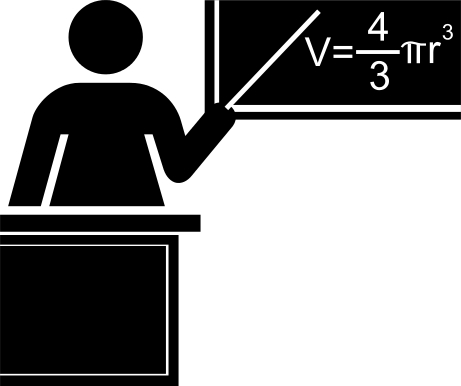
\includegraphics[width=.07\textwidth]{teacher.jpg} & 
\begin{minipage}{.85\textwidth}
}{%
\end{minipage}\\
\hline
\end{tabular}
}


%pour les fichiers c et dossiers
\newcounter{exoo} \setcounter{exoo}{0}
\newcommand{\numexo}{\theexoo}
\newcommand{\repexo}{{\tt exo\_\numexo}}
\newcommand{\exoplus}{\addtocounter{exoo}{1}}




\begin{document}
\maketitle





\thispagestyle{empty}


\section{Empilements}

\begin{action}
\item {\bf Prise en main - \tt empilements0.} Lisez le code et exécutez-le. Cet exercice utilise une mini-bibliothèque {\tt libEmpilements} 
qui étend {\tt tkiteasy} ; les exercices qui suivent seront faits sur le même modèle.
L'objectif de cette question est seulement de comprendre l'utilisation de la méthode {\tt empilerCube}. 
Modifiez librement le script en ajoutant des cubes supplémentaires empilés avec les premiers ou sur des espaces vides.
\item {\bf Trois fonctions - \tt empilements1.} Ce script définit trois fonctions qui s'appellent entre elles. L'objectif ici
est de comprendre en regardant le code pourquoi les cubes tombent exactement dans cet ordre et sur ces positions.
\item {\bf Sans tricher ! - \tt empilements2.} Si vous avez compris, essayez de prévoir 
dans quel ordre et à quels endroits vont tomber les cubes si l'ont fait l'appel de fonction {\tt fa(g,2)} (il faut l'ajouter). Prenez un papier et essayez
de noter dans quel ordre tombent les cubes, sur quel emplacement et avec quelle couleur ! Si vous vous êtes trompé, 
ce n'est pas grave mais essayez de comprendre pourquoi !
\item {\bf Cette fois-ci, vraiment sans tricher ! - \tt empilements3.} Même exercice si l'on ajoute dans ce script l'appel de fonction {\tt fA(g,2)}.
\item {\bf Chassé-croisé - \tt empilements4.}  Essayez de prévoir ce que va faire l'appel {\tt f0(g,0)}.
\item {\bf suite - \tt empilements4.} A la fin de la fonction {\tt f0}, ajoutez l'empilement d'un cube rouge sur la même
position que le cube bleu. Comment et dans quel ordre cela va-t'il se passer ?
\end{action}

\begin{icone}{img/lecture.jpg}
  Dans l'exercice précédent, vous avez vu deux fonctions {\tt f0} et {\tt f1} qui s'appellent l'une l'autre. Il ne nous
  reste plus beaucoup de chemin à faire pour utiliser maintenant une fonction qui s'appelle elle-même : une fonction {\it récursive}.

  Attention : dans les exercices ci-dessous, celle ou celui qui écrit une boucle va au coin !
\end{icone}


\begin{action}
\item {\bf Première fonction récursive - \tt empilements5}. La fonction qui effectue le travail d'empilement de cubes est la fonction {\tt f0}. 
Comme vous le voyez cette fonction ne contient pas de boucle.  La ligne où la fonction {\tt f0}
appelle la fonction {\tt f0} dans son propre code est \emph{l'appel récursif}. 
\item {\bf Suite - \tt empilements5}. Déplacez l'appel récursif \emph{avant} l'empilement. Que se passe-til ? Expliquez !
\item {\bf Suite - \tt empilements5}. Modifiez le code afin d'empiler un cube bleu de gauche à droite, puis un cube vert
de droite à gauche, avec un seul appel récursif !
\item {\bf A vous - \tt empilements6}. Sur le modèle de l'exercice précédent, écrivez une fonction récursive mais qui
fasse une récurrence descendante, de la position 9 à la position 0 en empilant des cubes. Puis modifiez le code afin
d'obtenir un empilement de droite à gauche, suivit d'une seconde ligne de gauche à droite (toujours un seul appel récursif.)
\item {\bf remplissage - \tt empilements7 } La fonction {\tt f0} de l'exercice précédent, dans sa première version permettait de remplir
toute une ligne. Pouvez-vous créer une deuxième fonction qui va appeler {\tt f0} pour remplir une ligne, 
puis qui va s'appeler elle-même afin de remplir la ligne du-dessus ? Si cela fonctionne, tout l'écran sera rempli par récurrence.
Attention, il faut s'arrêter à un moment quand les lignes deviennent trop hautes (vous pouvez avoir besoin d'un compteur).
\end{action}




\end{document}
